\Chapter{Tesztelés}

\Section{Használat}
A program használata egyszerű. Futtatás után a weboldalon kiválasztjuk a feldolgozandó fájlt. Innentől a program automatikusan működik. Ezután ki lehet választani a menüsávban a kívánt menüpontokat, amik átirányítanak a megfelelő oldalakra. Az első menüpont az architektúra, a második a kód oldal, harmadik a szimuláció. A kezdőoldalra a Szakdolgozatra kattintva lehet visszajutni. A kód oldalon a Gannt diagram elemeire kattintva lehet az egyes kódsorokat jobban megvizsgálni. A szimuláció oldalon lehet az aritmetikát vizsgálni, valamint saját szimulációt készíteni. Saját szimulációhoz útmutató a mellékelt Instruction Guide.txt és a Custom Instructions Example.txt

\Section{Tesztek}
A program az indulást követően szinte valós idejű, a szimulációra és a hardware szolgáltatásokra kell esetekben várni 1-2 másodpercet. Memória igény felső korlátja 160MB + a böngésző memóriaigénye, tárhely igény 3 MB.

A program működését a sum array minta programon keresztül kerül tesztelésre. A webalkalmazás elindítását követően megjelenik a kezdőoldal ahol fel tudjuk tölteni a kiválasztott fájlunkat, fájljainkat.

\begin{figure}[h]
\centering
\frame{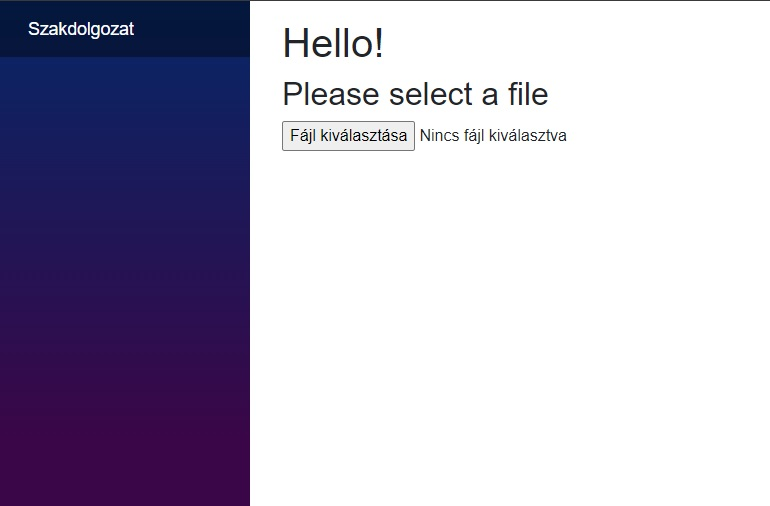
\includegraphics[scale=0.7]{images/Start.jpg}}
\caption{Webalkalmazás kezdő állapota}
\label{fig:start}
\end{figure}

\newpage
Feltöltést követően a háttérben rögtön lezajlik a fájl elemzése, szimulációk, kimutatások készítése. Amíg ez történik, a felhasználói felület nem válaszol, de az utasításokat eltárolja, tehát ha rögtön rákattintunk az architektúra fülre, minimális késleltetés után betölti a lapot.

\begin{figure}[h]
\centering
\frame{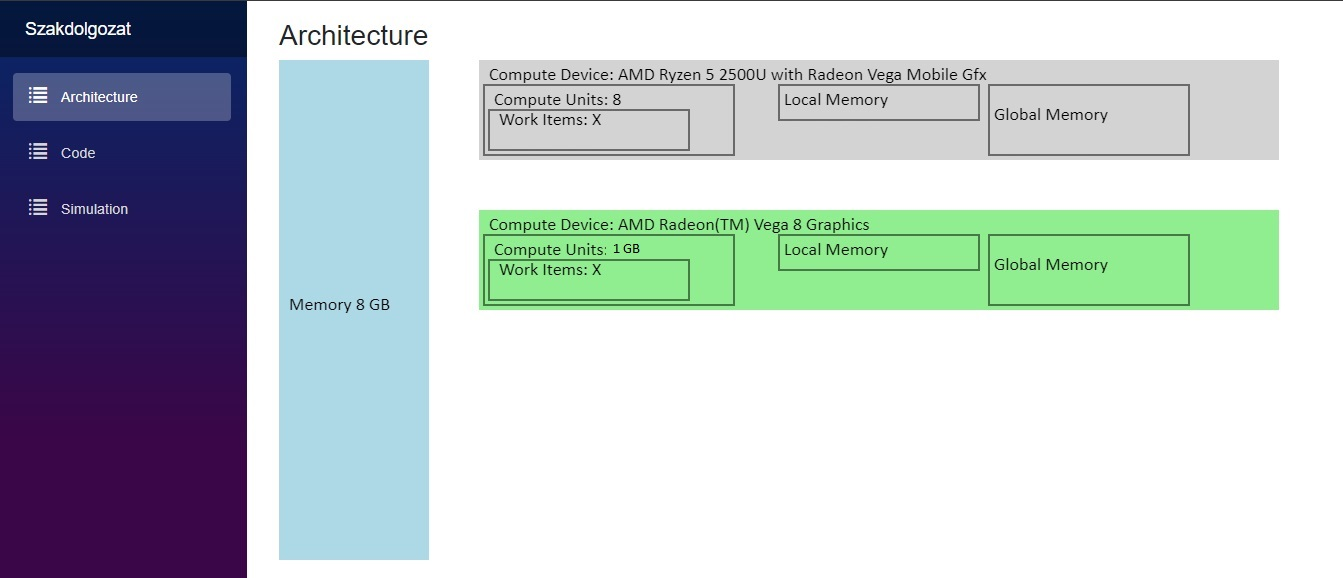
\includegraphics[scale=0.4]{images/Architecture.jpg}}
\caption{Architekture oldal}
\label{fig:arch}
\end{figure}


Az architektúra lapon látszódik az elérhető rendszer memória nagysága, a processzor neve, magjainak száma azaz a számítási egységeinek a száma. Megjeleníti még a videokártya nevét, és elérhető videómemóriát a számítási egységek helyén. Ez a videokártya számítási egységeinek megszámlálhatatlansága miatt történik.

\begin{figure}[h]
\centering
\frame{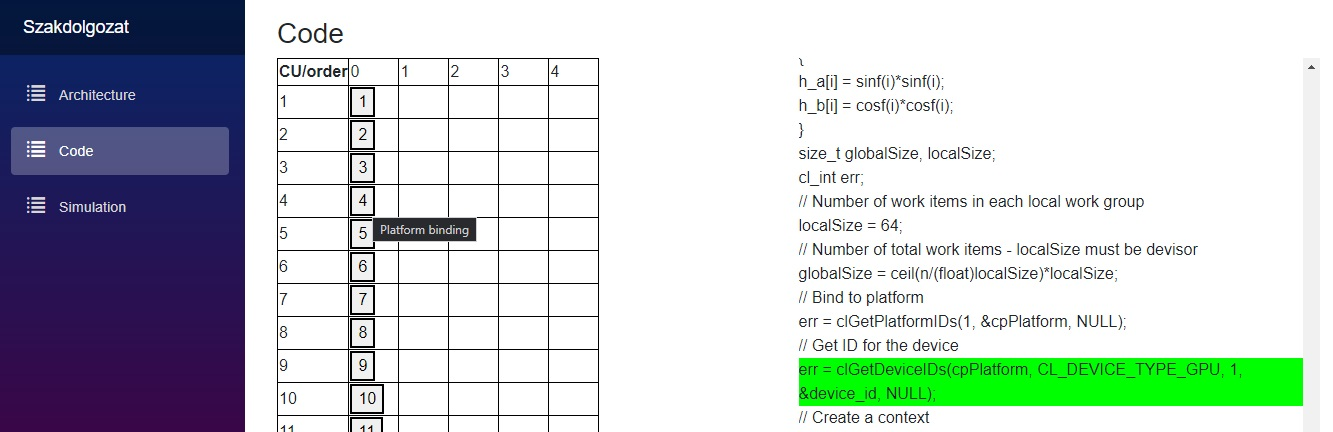
\includegraphics[scale=0.4]{images/Code.jpg}}
\caption{Code oldal}
\label{fig:code}
\end{figure}

\newpage
A Code menüpontra kattintva a következő oldalra jutunk. Itt láthatók forrásfájlban található OpenCL utasítások, eljárások, táblázatos formában attól függően hogy melyik Számítási egységen futnak. 0 jelöli a processzoron történő szekvenciális futást, a maradék számok pedig párhuzamos résznél jelzik hogy melyik számítási egységeken fut az OpenCL kernel. Mivel a példában használt OpenCL eszköz a videókártya, ezért a program nem tudja megállapítani a számítási egységek mennyiségét, tehát az alapértelmezett 4 db számítási egységgel számol. Az egeret egy elemre pozicionálva információt kapunk az adott elemről, rákattintva pedig a táblázat mellett lévő kód részletben a megfelelő sorra teker és kiemeli azt.

\begin{figure}[h]
\centering
\frame{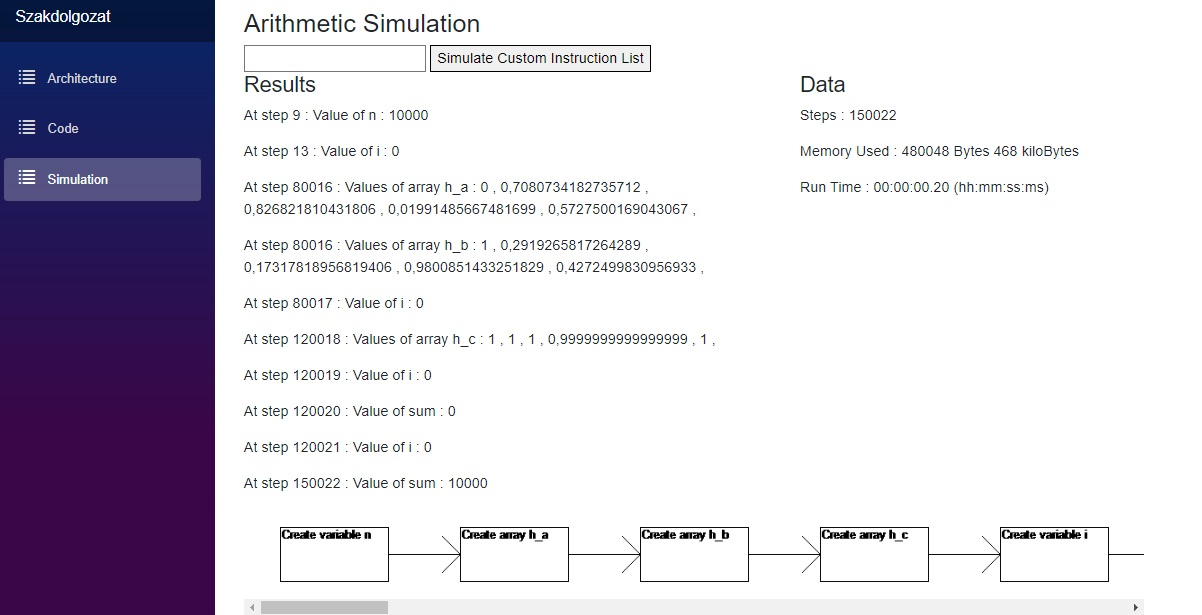
\includegraphics[scale=0.44]{images/Simulation.jpg}}
\caption{Simulation oldal}
\label{fig:sim}
\end{figure}


A Simulation menüre kattintva megnyílik a szimuláció oldala, ahol látható a szimuláció fontosabb lépéseinek eredményei, mint az értékadások és a végeredmény. Az oldal jobb oldalán láthatóak a szimuláció adatai, mint a minimum memóriaigény, lépésszám, futási idő, globális és lokális méret, munka csoportok száma, és a használt eszköz. Az oldal alján látható a szintaxis fa, tekerhető, minden nyíl korrekt. Egy szimulációs eredményt a szintaxis fához tudunk viszonyítani az azonosító (\#) számuk megfeleltetésével.
Az oldal tetején megjelenik a saját instrukciós lista futtatása felület, ami hiba nélkül működik.